\documentclass[aspectratio=43,12pt]{beamer}
\usepackage{tabularx}
\usepackage{array}
\usepackage{graphicx}
\usepackage{listings}
\usepackage{hyperref}
\usepackage{color}
\usepackage{tikz}
\usetikzlibrary{arrows.meta, positioning, shapes.geometric,matrix}
\usecolortheme{whale}
\setbeamertemplate{itemize subitem}{\small$\bullet$}
\definecolor{lightgray}{gray}{0.95}
\setbeamerfont{section in toc}{size=\small}
\setbeamerfont{subsection in toc}{size=\scriptsize}
\lstset{
    language=SQL,
    showspaces=false, 
    numbers=left,
    numberstyle=\tiny,
    backgroundcolor=\color{lightgray},
    keywordstyle=\color{blue}\bfseries,
    commentstyle=\color{gray},
    stringstyle=\color{orange},
    basicstyle=\ttfamily\scriptsize,
    breaklines=true,
    literate=
        {é}{{\'e}}1
        {è}{{\`e}}1
        {à}{{\`a}}1
        {ù}{{\`u}}1
        {ç}{{\c{c}}}1
        {ô}{{\^o}}1
        {ê}{{\^e}}1,
}


\newcommand{\paren}[1]{\left(#1\right)} % (x)


\title[Optimisation du plan et de l’exécution de requêtes SQL]{Optimisation du temps d'éxécution des requêtes SQL}
\author{Eliott PAQUET N° 30960}
\date{2025 -- 2026}
    

% Barre Pied de page
\setbeamertemplate{footline}{
    \begin{beamercolorbox}[wd=\paperwidth,ht=2.5ex,dp=1ex]{author in head/foot}
    \usebeamerfont{author in head/foot}
    \hspace*{2ex}\insertauthor\hfill \insertshorttitle\hfill \insertdate\hfill \insertframenumber/\inserttotalframenumber\hspace*{2ex}
    \end{beamercolorbox}
}

% Barre d'en tête
\setbeamertemplate{headline}{%
    \begin{beamercolorbox}[ht=2.5ex,dp=1.125ex,center]{section in head/foot}
        \insertsection
    \end{beamercolorbox}%
}

\begin{document}
\begin{frame}
    \titlepage
\end{frame}

\begin{frame}
    \frametitle{Sommaire}
    \tableofcontents[hideothersubsections]

\end{frame}


\section{Les bases du traitement des requêtes SQL}
\subsection{Introduction}
\begin{frame}{Chiffres clés sur l'utilisation de SQL}

    \begin{itemize}

        \item \textbf{Amazon Aurora}
              \begin{itemize}
                  \item Jusqu'à \textbf{500 000 lectures/sec} et \textbf{100 000 écritures/sec}
                  \item Soit environ \textbf{600 000 requêtes SQL par seconde}
                  \item $\approx$ \textbf{51 milliards de requêtes par jour}
                  \item Source : \url{https://aws.amazon.com/blogs/aws/now-available-amazon-aurora/}
              \end{itemize}

              \vspace{0.5cm}

        \item \textbf{Oracle Database (Exadata)}
              \begin{itemize}
                  \item Jusqu'à \textbf{1 million de transactions par seconde}
                  \item $\approx$ \textbf{86 milliards de requêtes par jour}
                  \item Source : benchmark Exadata (IT Convergence)
              \end{itemize}
    \end{itemize}

\end{frame}

\subsection{L'algèbre relationnelle}
\begin{frame}[fragile]
    \frametitle{Edgar F. Codd (1970/1971)}

    \centering
    Calcul relationnel \(\Longleftrightarrow\) Algèbre relationnelle \hspace{1 em}

    \vspace{0.5cm}

    \begin{minipage}{0.48\textwidth}
        \begin{lstlisting}[language=SQL]
SELECT S.Id, S.Price
FROM Sales
JOIN Dp ON Dp.Id = S.DpId
WHERE Dp.Name = 'Morbihan';
            \end{lstlisting}
    \end{minipage}
    \hfill
    \begin{minipage}{0.48\textwidth}
        \centering
        \begin{tikzpicture}[
                scale=0.85,
                transform shape,
                node distance=1cm,
                block/.style={minimum width=1cm, minimum height=1cm, align=center},
                arrow/.style={-Stealth, thick}
            ]

            % Opérateurs
            \node[block] (pi) {$\Pi_{Sales.Id,\,Sales.Price}$};
            \node[block, below=of pi] (sigma) {$\sigma_{Dp.Name = \text{'Morbihan'}}$};
            \node[block, below=of sigma] (join) {$\Join_{Dp.Id = Sales.DpId}$};

            % Relations
            \node[block, below left=of join] (sales) {$Sales$};
            \node[block, below right=of join] (dp) {$Dp$};

            % Flèches
            \draw[arrow] (sigma) -- (pi);
            \draw[arrow] (join) -- (sigma);
            \draw[arrow] (sales) -- (join);
            \draw[arrow] (dp) -- (join);

        \end{tikzpicture}
    \end{minipage}
\end{frame}
\begin{frame}{Problématique}
    \begin{center}
        \underline{\textbf{Comment créer, optimiser et éxécuter un plan de requête ?}}
    \end{center}
    \begin{figure}[h]
        \centering
        
\includegraphics[width=300pt]{../ressource/query_map.png}
        \caption{Traitement d'une requête SQL par un SGBD.}
        \vspace{2mm}
        Source : \href{https://blog.quest.com/sql-server-execution-plan-what-is-it-and-how-does-it-help-with-performance-problems/}{Quest}
    \end{figure}
\end{frame}
\section{Implémentation d'un Algebrizer en c++}
\begin{frame}{Les informations disponibles à l'entrée de l'algebrizer}
    \begin{itemize}
        \item \textbf{Parser}
              \begin{itemize}
                  \item Colonne selectionné
                  \item Différente Jointures
                  \item Condition
                  \item Group By /Agrégation
              \end{itemize}
        \item \textbf{Mémoire}
              \begin{itemize}
                  \item différentes Tables/Colonnes
                  \item Nombre de ligne
                  \item autres statistiques (tri,indexation,cracking)
              \end{itemize}
    \end{itemize}
\end{frame}
\begin{frame}{Arbre Naïf}
    \centering
    \begin{tikzpicture}[
            scale=0.85,
            transform shape,
            node distance=0.3cm,
            block/.style={minimum width=1cm, minimum height=1cm, align=center},
            arrow/.style={-Stealth, thick}
        ]

        \node[block] (aleph) {$\aleph_{\gamma_{\paren{\text{Sales.Id}}}, \varphi_{\paren{\text{Sales.Price}}}}$};

        \node[block, below=of aleph] (pi) {$\Pi_{\text{Sales.Id},\,\text{Sales.Price}}$};

        \node[block, below=of pi] (sigma) {$\sigma_{\text{Dp.Name} = \text{'Morbihan'} \text{ et } \text{employe.name} = \text{'Eliott'} \text{ et } \text{Customer.Name} = \text{'Antoine'}}$};

        \node[block, below=of sigma] (joinMain) {$\Join_{\text{Sales.IdVendeur} = \text{Employe.Id}}$};

        \node[block, below left=of joinMain,xshift=1cm] (joinCust) {$\Join_{\text{Sales.CustomerId} = \text{Customer.Id}}$};

        \node[block, below right=of joinMain,xshift=-1cm] (joinDir) {$\Join_{\text{Dp.Id} = \text{employé.IdDp}}$};

        \node[block, below left=of joinCust, xshift=1cm] (sales) {$Sales$};
        \node[block, below right=of joinCust, xshift=-1cm] (customer) {$Customer$};

        \node[block, below right=of joinDir, xshift=-1cm] (dp) {$Dp$};
        \node[block, below left=of joinDir,xshift=1cm] (employé) {$employe$};

        \draw[arrow] (pi) -- (aleph);
        \draw[arrow] (sigma) -- (pi);
        \draw[arrow] (joinMain) -- (sigma);

        \draw[arrow] (joinCust) -- (joinMain);
        \draw[arrow] (joinDir) -- (joinMain);

        \draw[arrow] (sales) -- (joinCust);
        \draw[arrow] (customer) -- (joinCust);

        \draw[arrow] (dp) -- (joinDir);
        \draw[arrow] (employé) -- (joinDir);


    \end{tikzpicture}

\end{frame}
\section{La gestion mémoire}
\begin{frame}
    \frametitle{Les bases de données orientées colonnes}
    \begin{figure}[h]
        \centering
        
\includegraphics[width=300pt]{../ressource/row_vs_column.png}
        \caption{Rendu physique des BDD orientées colonnes et BDD orientées lignes}
    \end{figure}
\end{frame}
\subsection{Optimisation mémoire}
\begin{frame}{Optimisation mémoire}
    \centering
    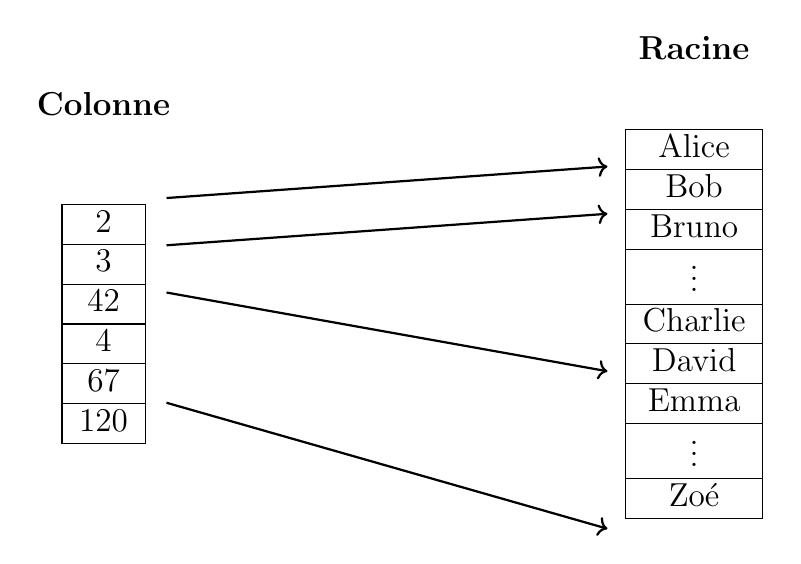
\begin{tikzpicture}[
            every node/.style={font=\large}
        ]

        \node at (-0.5,2.8) {\textbf{Colonne}};
        \node at (7,3.5) {\textbf{Racine}};

        \node (left) at (-0.5,0) {
            \begin{tabular}{|c|}
                \hline
                2   \\ \hline
                3   \\ \hline
                42  \\ \hline
                4   \\ \hline
                67  \\ \hline
                120 \\ \hline
            \end{tabular}
        };

        \node (right) at (7,0) {
            \begin{tabular}{|c|}
                \hline
                Alice    \\ \hline
                Bob      \\ \hline
                Bruno    \\ \hline
                $\vdots$ \\ \hline
                Charlie  \\ \hline
                David    \\ \hline
                Emma     \\ \hline
                $\vdots$ \\ \hline
                Zoé      \\ \hline
            \end{tabular}
        };

        \draw[->, thick] (0.3,1.6) -- (5.9,2);
        \draw[->, thick] (0.3,1) -- (5.9,1.4);
        \draw[->, thick] (0.3,0.4) -- (5.9,-0.6);
        \draw[->, thick] (0.3,-1) -- (5.9,-2.6  );

    \end{tikzpicture}

\end{frame}
\begin{frame}{Notre Premier Modèle}
    \begin{center}
        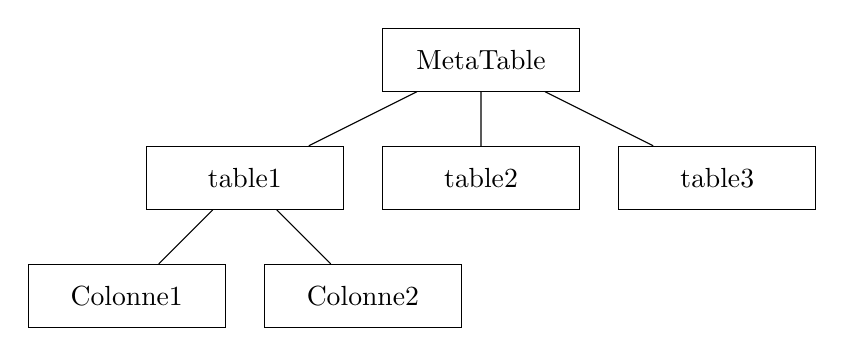
\begin{tikzpicture}[
                level distance=1.5cm,
                sibling distance=3cm,
                every node/.style={draw, rectangle, align=center, minimum width=2.5cm, minimum height=0.8cm}
            ]

            % Racine de l'arbre
            \node {MetaTable}
            % Niveau 1 : les tables
            child { node {table1}
                    % Niveau 2 : colonnes de table1
                    child { node {Colonne1} }
                    child { node {Colonne2} }
                }
            child { node {table2} }
            child { node {table3} };
        \end{tikzpicture}
    \end{center}

    \begin{itemize}
        \item \textbf{Colonne} : Racine et liste de position dans la racine encore valide
        \item \textbf{Table} : liste de Colonne encore valide
        \item \textbf{MetaTable} : Liste de plusieurs \textit{Tables}.
        \item \textbf{Particularité} : à une même position, les valeurs des colonnes forment une ligne de donnée
    \end{itemize}
\end{frame}
\begin{frame}{Application sur nos opérations}
    \begin{tikzpicture}

        \node at (0.25,3.5) {\textbf{Selection}};
        \node at (7,3.5) {\textbf{Jointure}};

        \node at (-1,0) {
            \begin{tabular}{|c|}
                \hline
                2   \\ \hline
                3   \\ \hline
                42  \\ \hline
                35  \\ \hline
                12  \\ \hline
                98  \\ \hline
                67  \\ \hline
                420 \\ \hline
            \end{tabular}
        };
        \node at (1.5,0) {
            \begin{tabular}{|c|}
                \hline
                2   \\ \hline
                67  \\ \hline
                420 \\ \hline
            \end{tabular}
        };
        \draw [line width=1pt, double distance=3pt,arrows = {-Latex[length=0pt 3 0]}] (-0.25,0) -- (0.8,0);

        \node at (5,0) {$\Join$};
        \node at (4.25,0) {
            \begin{tabular}{|c|}
                \hline
                2   \\ \hline
                3   \\ \hline
                42  \\ \hline
                35  \\ \hline
                12  \\ \hline
                98  \\ \hline
                67  \\ \hline
                420 \\ \hline
            \end{tabular}
        };
        \node at (5.75,0) {
            \begin{tabular}{|c|}
                \hline
                54  \\ \hline
                78  \\ \hline
                904 \\ \hline
            \end{tabular}
        };

        \node at (8.5,0) {
            \begin{tabular}{|c|c|}
                \hline
                2   & 78  \\ \hline
                3   & 54  \\ \hline
                3   & 78  \\ \hline
                3   & 904 \\ \hline
                98  & 78  \\ \hline
                98  & 904 \\ \hline
                420 & 54  \\ \hline
            \end{tabular}
        };
        \draw [line width=1pt, double distance=3pt,arrows = {-Latex[length=0pt 3 0]}] (6.5,0) -- (7.35,0);
    \end{tikzpicture}
\end{frame}


\subsection{Limites de notre premier modèle}
\begin{frame}{Invariant lors de l'exécution}
    \underline{Les lignes} formé par la concaténation de toutes les colonnes d'une \underline{Meta-Table restent les mêmes jusqu'à la fin}
    ~\\~\\
    \underline{Les lignes} formé par la concaténation de toutes les colonne d'une \underline{Table sont les même à l'initalisation}
    ~\\~\\  ~\\~\\

    \underline{Les Colonnes d'une même table sont des doublons !}

\end{frame}
\begin{frame}{Optimisation de notre modèle}
    \begin{center}
        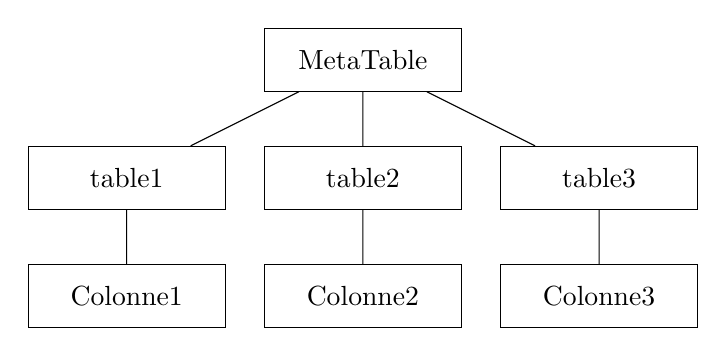
\begin{tikzpicture}[
                level distance=1.5cm,
                sibling distance=3cm,
                every node/.style={draw, rectangle, align=center, minimum width=2.5cm, minimum height=0.8cm}
            ]

            % Racine de l'arbre
            \node {MetaTable}
            % Niveau 1 : les tables
            child { node {table1}
                    % Niveau 2 : racines de table1
                    child { node {Colonne1} }
                }
            child {
                    node {table2}
                    child { node {Colonne2} }
                }
            child {
                    node {table3}
                    child { node {Colonne3} }};
        \end{tikzpicture}
    \end{center}

    \begin{itemize}
        \item \textbf{Particularité} : Une colonne par table (ne dépend pas du nombre de colonnes)
        \item \textbf{ Résultat} : \(45\) min \(\to\) \(22\) secondes
    \end{itemize}
\end{frame}

\section{Optimisation du plan}
\subsection{Quelques optimisation naïves}
\begin{frame}{Quelques Optimisation de l'arbre Naïf}
    \begin{itemize}
        \item Descente de sélection
        \item Ajout de projection
    \end{itemize}
    Graphe présentant les 3 versions en fonction de la taille du jeux de donnée
\end{frame}

\subsection{Méthodes de jointure}
\begin{frame}
    \frametitle{Les différents types de jointures possibles}
    \begin{itemize}
        \item Produit Cartésien : \( \mathcal{O}(n \times m)\)\\
        \item Jointure Triée :  \( \mathcal{O}(n \log(n) + n + m\log(m) +m)\)
        \item Jointure par dictionnaire : \( \mathcal{O}(2n)\)
    \end{itemize}
    graphe présentant les 3 type de jointure en fonction du nombre de données
\end{frame}

\section{Optimisation dépendante des données}
\subsection{Optimisation des expressions binaires}
\begin{frame}[fragile]
    \frametitle{Analyse des expressions binaires}

    % Query en haut
    \begin{lstlisting}[language=SQL]
WHERE (Dep.pays = "France" AND Sales.Id = 543) OR (Product.Origine = "Chine")
    \end{lstlisting}

    \vspace{0.5cm} % petit espace entre query et arbre

    % Arbre en dessous
    \begin{center}
        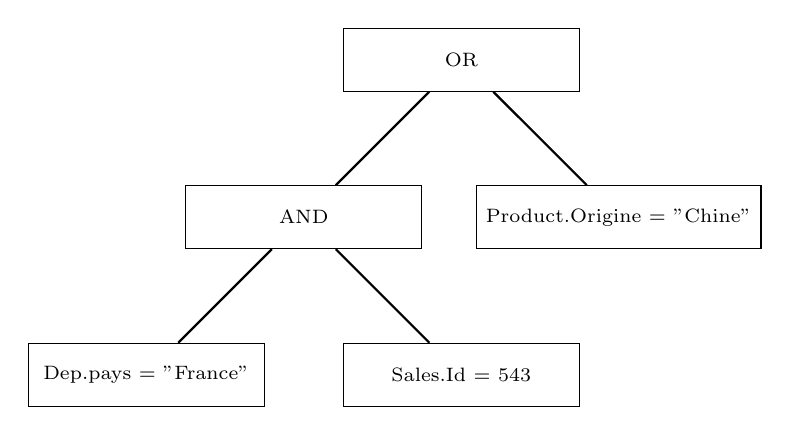
\begin{tikzpicture}[
                scale=1,
                level distance=2cm,
                sibling distance=4cm,
                every node/.style={draw, rectangle, align=center, minimum width=3cm, minimum height=0.8cm, font=\scriptsize},
                arrow/.style={-, thick}]
            % Arbre
            \node (or) {OR}
            child { node (and) {AND}
                    child { node (cond1) {Dep.pays = "France"} }
                    child { node (cond2) {Sales.Id = 543} }
                }
            child { node (cond3) {Product.Origine = "Chine"} };

            % Flèches parcours préfixe (parent → enfants)
            \draw[arrow] (or) -- (and);
            \draw[arrow] (and) -- (cond1);
            \draw[arrow] (and) -- (cond2);
            \draw[arrow] (or) -- (cond3);

        \end{tikzpicture}
    \end{center}
\end{frame}

\begin{frame}[fragile]
    \frametitle{Optimisation des expressions binaires}

    % Query en haut
    \begin{lstlisting}[language=SQL]
WHERE (Dep.pays = "France" AND Sales.Id = 543) OR (Product.Origine = "Chine")
    \end{lstlisting}

    \vspace{0.5cm} % petit espace entre query et arbre

    % Arbre en dessous
    \begin{center}
        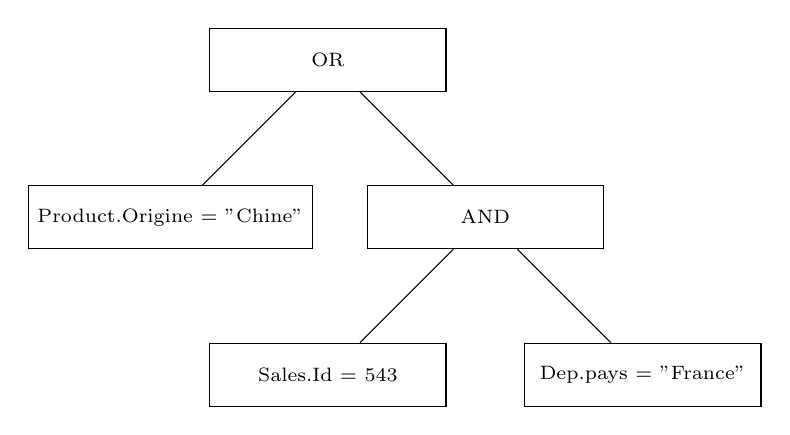
\begin{tikzpicture}[
                scale=1,
                level distance=2cm,
                sibling distance=4cm,
                every node/.style={draw, rectangle, align=center, minimum width=3cm, minimum height=0.8cm, font=\scriptsize},
                arrow/.style={-, thick}]

            % Arbre
            \node (or) {OR}

            child { node (cond3) {Product.Origine = "Chine"} }
            child { node (and) {AND}
                    child { node (cond2) {Sales.Id = 543} }
                    child { node (cond1) {Dep.pays = "France"} }
                };

        \end{tikzpicture}
    \end{center}

\end{frame}

\begin{frame}
    graphe opti binaire
\end{frame}

\subsection{Choix de l'ordre des jointures}
\begin{frame}
    \frametitle{Résultats équivalents mais complexité différente}

    \begin{minipage}{0.48\textwidth}
        \begin{tikzpicture}[
                scale=0.7,
                transform shape,
                node distance=0.6cm and 0cm,
                block/.style={minimum width=0.6cm, minimum height=0.6cm, align=center},
                arrow/.style={-Stealth, thick},
                card/.style={font=\scriptsize, above}
            ]

            % Jointures
            \node[block] (join1) {$\Join_{Dp.Id = Sales.DpId}$};
            \node[card] at (join1.north) {$10^2$};

            \node[block, below left=0.8cm and -1cm of join1] (join2)
            {$\Join_{Sales.ProductId = Product.Id}$};
            \node[card] at (join2.north) {$10^6$};

            % Relations
            \node[block, below left=0.8cm and -1cm of join2] (sales) {$Sales$};
            \node[card] at (sales.north) {$10^6$};

            \node[block, below right=0.8cm and -1cm of join2] (product) {$Product$};
            \node[card] at (product.north) {$10^4$};

            \node[block, below right=0.8cm and -1cm of join1] (dp) {$Dp$};
            \node[card] at (dp.north) {$1$};

            % Flèches
            \draw[arrow] (join2) -- (join1);
            \draw[arrow] (sales) -- (join2);
            \draw[arrow] (product) -- (join2);
            \draw[arrow] (dp) -- (join1);

        \end{tikzpicture}
    \end{minipage}
    \begin{minipage}{0.48\textwidth}
        \begin{tikzpicture}[
                scale=0.7,
                transform shape,
                node distance=0.6cm and 0cm,
                block/.style={minimum width=0.6cm, minimum height=0.6cm, align=center},
                arrow/.style={-Stealth, thick},
                card/.style={font=\scriptsize, above}
            ]

            % Jointures
            \node[block] (join1) {$\Join_{Sales.ProductId = Product.Id}$};
            \node[card] at (join1.north) {$10^2$};

            \node[block, below left=0.8cm and -1cm of join1] (join2)
            {$\Join_{Dp.Id = Sales.DpId}$};
            \node[card] at (join2.north) {$10^2$};

            % Relations
            \node[block, below left=0.8cm and -1cm of join2] (sales) {$Sales$};
            \node[card] at (sales.north) {$10^6$};

            \node[block, below right=0.8cm and -1cm of join1] (product) {$Product$};
            \node[card] at (product.north) {$10^4$};

            \node[block, below right=0.8cm and -1cm of join2] (dp) {$Dp$};
            \node[card] at (dp.north) {$1$};

            % Flèches
            \draw[arrow] (join2) -- (join1);
            \draw[arrow] (sales) -- (join2);
            \draw[arrow] (product) -- (join1);
            \draw[arrow] (dp) -- (join2);

        \end{tikzpicture}
    \end{minipage}


    \vspace{1cm}
    \begin{itemize}
        \item \(\Join_{Sales.ProductId = Product.Id}\) d'abord → \(10^4\times10^6 + 10^6 \times 1 \) comparaisons
        \item \(\Join_{Dp.Id = Sales.DpId}\) d'abord \(\rightarrow\) \(1\times10^6 + 10^2 \times 10^4 \) comparaisons
    \end{itemize}

\end{frame}

\begin{frame}{Comment choisir l'ordre ?}
    {\textbf{Mon Algorithme}}
    BUT : Minimiser à tout moment le nombre de ligne
    ~\\~\\
    Def : Rapport de Cardinalité \( \to \frac{\text{Estimation du nombre de ligne créé}}{\text{produit du nombre de ligne testé}}\)
    ~\\~\\\begin{enumerate}
        \item Calcul le RC de chaque Jointure
        \item Trie les Jointure par RC croissant
        \item Ajoute les jointures une par une à l'aide de notre structure Union-Find sur les tables
    \end{enumerate}
\end{frame}

\begin{frame}
    graphe ordre de jointure
\end{frame}
\section{analyse des résultats}
\begin{frame}
    \frametitle{Analyse de toutes les optimisations}
    Graphe toute optimisation
\end{frame}
\section{Conclusion}
\subsection{Conclusion}
\begin{frame}
    \frametitle{Résumé}
    \begin{itemize}
        \item Création d'un Algebrizer pour transformer le SQL en des opérations éxécutables
        \item Optimisations de notre modèle de représentation mémoire
        \item Optimisation naïve de l'arbre naïf
        \item Optimisation dépendantes des données
    \end{itemize}
\end{frame}
\subsection{Ouverture}
\begin{frame}
    \frametitle{Ouverture}
    \textbf{Les pistes récentes :}
    \begin{itemize}
        \item Analyse des données \(\Rightarrow\) Machine Learning (Génération de plan, Choix de l'ordre des jointures, \dots)
        \item Une meilleure organisation des données en mémoire (Voire le travail d'Antoine)
        \item Les deux: \href{https://www.normalesup.org/~rouvroy/papers/NTU_25_QHICS.pdf}{\textit{Hypothetical Index Benefit Estimation on Column-oriented Databases using Quantiles} \(2025\)}

    \end{itemize}

\end{frame}
\subsection{Nos ressources}
\begin{frame}
    \frametitle{Nos ressources}
    \textbf{Nos ressources :}
    \begin{itemize}
        \item \href{https://drive.google.com/file/d/1KNmuRBf8CV-s-zqdkUEP8iyYlPgFiglb/view?usp=drive_link}{\textit{The Design and Implementation of Modern Column-Oriented Database Systems} \(2013\)}
        \item \href{https://web.stanford.edu/class/cs345d-01/rl/cstore.pdf}{\textit{C-Store: A Column-oriented DBMS} \(2005\)}
        \item \href{https://link.springer.com/content/pdf/10.1007/s41019-020-00149-7.pdf}{\textit{A Survey on Advancing the DBMS Query Optimizer: Cardinality Estimation, Cost Model, and Plan Enumeration} \(2021\)}
        \item \href{https://www.microsoft.com/en-us/research/wp-content/uploads/2024/12/Extensible-Query-Optimizers-in-Practice.pdf}{\textit{Extensible Query Optimizers in Practice} \(2024\)}
        \item \href{http://webdam.inria.fr/Alice/}{\textit{Foundation of Databases} \(1995\)}
    \end{itemize}
\end{frame}

\end{document}